%
% Annual Cognitive Science Conference
% Sample LaTeX Paper -- Proceedings Format
%

% Original : Ashwin Ram (ashwin@cc.gatech.edu)       04/01/1994
% Modified : Johanna Moore (jmoore@cs.pitt.edu)      03/17/1995
% Modified : David Noelle (noelle@ucsd.edu)          03/15/1996
% Modified : Pat Langley (langley@cs.stanford.edu)   01/26/1997
% Latex2e corrections by Ramin Charles Nakisa        01/28/1997
% Modified : Tina Eliassi-Rad (eliassi@cs.wisc.edu)  01/31/1998
% Modified : Trisha Yannuzzi (trisha@ircs.upenn.edu) 12/28/1999 (in process)
% Modified : Mary Ellen Foster (M.E.Foster@ed.ac.uk) 12/11/2000
% Modified : Ken Forbus                              01/23/2004
% Modified : Eli M. Silk (esilk@pitt.edu)            05/24/2005
% Modified: Niels Taatgen (taatgen@cmu.edu) 10/24/2006

%% Change ``a4paper'' in the following line to ``letterpaper'' if you are
%% producing a letter-format document.

\documentclass[10pt,letterpaper]{article}
\setlength{\belowcaptionskip}{5pt plus 3pt minus 2pt}
\usepackage{cogsci}
\usepackage{graphicx}
\usepackage{amsmath, amsthm, amssymb}
\usepackage{pslatex}
\usepackage{apacite}
\usepackage{multirow}
\usepackage{arydshln}
\usepackage{soul,color}
\usepackage{xspace}
%\usepackage[natbib=true]{biblatex}
\usepackage{natbib}
\usepackage{textcomp}
\usepackage[font = small]{caption}
\setlength{\belowcaptionskip}{-7pt}
\def\bibfont{\small}

\title{Present bias in exploratory choice}

\author{  {\large \bf Alexander S. Rich (asr443@nyu.edu)} \\ {\large\bf Todd M. Gureckis (todd.gureckis@nyu.edu)}\\
        New York University, Department of Psychology, 6 Washington Place, New York, NY 10003 USA}
\begin{document}
\maketitle

\begin{abstract}

  Balancing exploration and exploitation is difficult, and under-exploration
  appears to be a particularly pressing problem. We propose that one possible cause of
  under-exploration is present bias, in which immediate rewards (like those
  gained from exploitation) loom larger than future rewards (like those
  gained from exploration). This possible cause of under-exploration is not
  addressed by past lab studies, in which choices generally yield token rewards
  that are converted to money at the end of the experiment, removing the
  inter-temporal aspect of the decision-making process. In this paper, we
  develop an exploratory choice task with immediately-consumed rewards. In
  Experiment 1, we show that people understand the task and respond as expected
  to standard decision variables. In Experiment 2, we introduce a condition in
  which there is a temporal delay between choices and outcomes, and test whether
  this increases exploration by reducing present bias. While we find no effect
  of the delay, we discuss plans for future experiments to test the validity and
  robustness of this result.

  \textbf{Keywords} time preference, present bias, exploratory choice
\end{abstract}

Balancing exploitation of known options with exploration of known options
presents a difficult cognitive and motivational challenge. The problem of how to
trade off between these two conflicting goals has created whole fields of study
\citep{Mehlhorn2015, sutton1998reinforcement}, and in many cases achieving an
optimal balance is computationally intractible \citep{Guez2013}. Given these
facts, one might expect people to often deviate from optimal exploratory choice
in both directions, perhaps exploring too much in some situations but too little
in others.

Notably, though, while over-exploration does occur, a bias towards under-exploration in particular seems to be
observed across a wide range of domains. One of the most severe
expressions of under-exploration is learned helplessness, in which an organism
experiences the absence of contol over the environment, learns that the
environment is uncontrollable, and thus ceases to take actions that might allow
it to discover that it can in fact exert control. Learned helplessness has been proposed to
underly most notably depression \citep{Abramson1978, Abramson1989} but also
problems ranging from difficulties in school CITE to poverty CITE.
While the cognitive appraisal of experienced events affects the development of
learned helplessness \citep{Abramson1978}, patterns of exploration clearly play
a role as well \citep{Huys2009, Teodorescu2014a}. In the case of depression,
interventions aimed at increasing the exploration of activities this might
produce a sense of pleasure and mastery have been found to be as effective as
those with a more cognitive orientation \citep{Jacobson1996}.

Under-exploration also seems to occur in the development of complex skills, such
as flying a plane or playing a sport CITE. In these settings, an ``emphasis
change'' training method in which the focus of practice is repeatedly changed
can lead to greater performance gains than unguided practice or more complex
training methods. Emphasis change works because it encourages people to
continually explore the performance space to find more effective cognitive and
motor routines CITE. Without these interventions, people often enter a ``local
maximum'' in which exploration decreases and performance plateaus CITE.

There are many other areas in which under-exploration is less clearly
established, but is suspected to play a role in maladaptive behavior.
Insufficient exploratory interaction with outgroups may be one cause of
stereotypes and prejudice \citep{Denrell2005most}, and interventions that
increase inter-group contact reduce stereotypes \citep{Shook2008}. The crowding
out of exploration by exploitation is a concern in organizational behavior as
well \citep{March1991, Levinthal1993}, prompting research into organizational
structures that may preserve exploration \citep{Fang2010}.

\subsection{Under- and over-exploration in the lab}

Given the seeming pervasiveness of under-exploration in real-world decision
making, one might expect a clear pattern of under-exploration in lab
experiments. Instead, however, lab results are mixed, with people sometimes
under-exploring, sometimes over-exploring, and sometimes exploring close to an
optimal amount. To take two illustrative examples, \citet{Zwick2003} found that
in a sequential search task people under-searched when there were no information
costs but over-searched when there were information costs, and
\citet{Teodorescu2014} found that people explored unknown alternatives too often
or not often enough depending on whether rare outcomes were positive or
negative. Similar results have been obtained within and across a variety of
other studies and paradigms
\citep{tversky1966information, Busemeyer1988, hertwig2004decisions, Navarro2016, Juni2016, Sang2011}.

These experimental studies raise the question of why under-exploration appears
more widespread than over-exploration in the field, but not in the lab. One
possibility is that both forms of deviation from optimality are in fact
prevalent, though perhaps in different settings, and that the seemingly general bias
toward under-exploration is illusory. In the current paper, we propose an
alternative hypothesis: that lab tests of exploratory choice have been missing a key component
of real-world exploratory choice, namely, the distribution of choices and
outcomes over time, and that this spreading of exploratory choices over time may
account for the tendency to under-explore.

\begin{figure*}
\centering
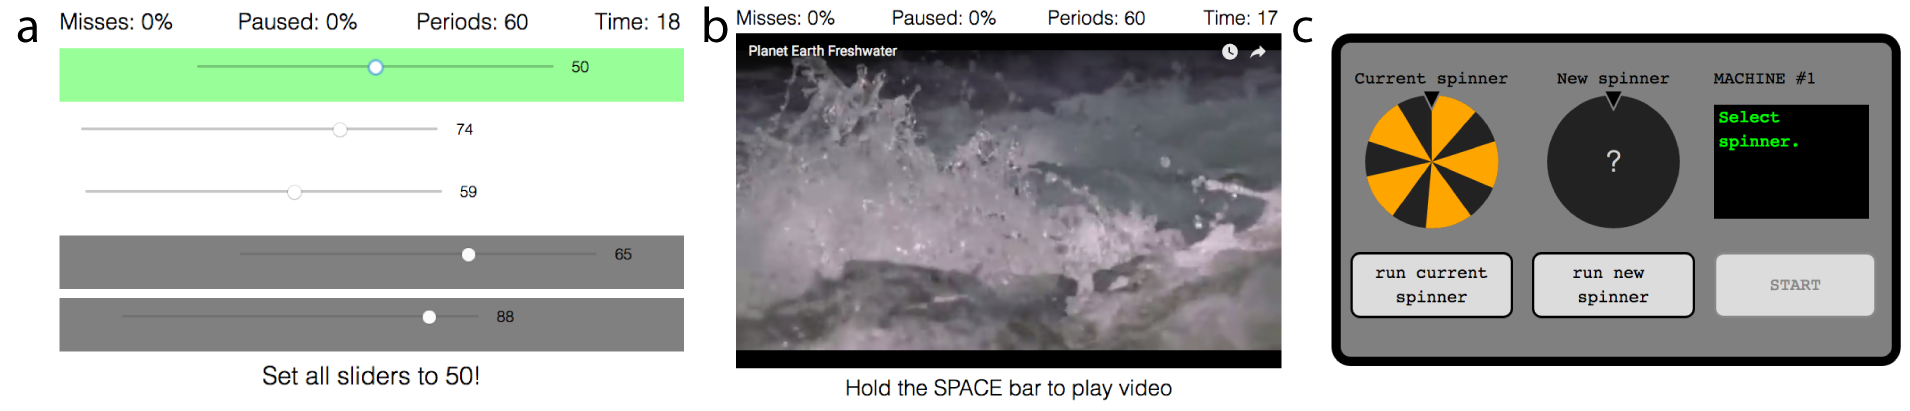
\includegraphics[width=\textwidth]{figures/taskpictures.png}
\caption{\emph{a}: An example of the slider task. Participants had to move all
  sliders to ``50'' in 30 seconds. \emph{b}: the video-watching task.
  Participants had to hold the space bar to watch their chosen video. \emph{c}:
  The decision-making task. Participants had to choose to run the machine with
  the current spinner or try a new spinner. If their chosen spinner landed on
  a gold wedge, they performed the video-watching task instead of the
  slider task.}
\label{fig:taskpictures}
\end{figure*}

\subsection{Exploration and myopia}

Under-exploration is often proposed to be the result of myopia: the
underweighting of temporally distant rewards relative to close ones \citep{March1991, Levinthal1993}. While
choosing actions that are expected to immediately maximize reward is inherently
exploitative, exploration often requires the decision-maker to suffer short-term
costs in search of better future options.

There are two distinct possible causes of myopia \citep{Bartels2015}. The first is that the decision-maker is
unaware of or fails to consider the future. This form of myopia is likely one
cause of under-exploration, particularly in complex environments. However,
researchers in exploratory choice have begun to address this form of myopia, and
have found that people change their
patterns of exploration based on their expectations about future choices,
showing that, at least to some degree they do consider the future \citep{Meyer1995, Wilson2014a, Rich2017}.

The the second form of myopia is that the decision-maker
is aware of the future but simply doesn't care as much about it.
A wealth have studies have shown that this form of myopia is an important factor
in human decision making, and that people are strongly
biased towards  the present. For example, people will often prefer a larger, later monetary
reward to a smaller, sooner reward when both rewards are in the future, but will
switch their preference when the time until both rewards is reduced so that the
sooner reward is immediate \citep{Kirby1995}. With monetary rewards, the delay
or speed-up required to observe preference reversals is usually several days. With non-monetary rewards,
such as the cessation of an annoying noise \citep{Solnick1980}, watching a video
when bored \citep{Navarick1998}, or drinking soda
when thirsty \citep{Brown2009}, a bias towards immediate rewards has been observed on the scale of
minutes or even seconds.

Present bias has the clear potential to cause people to explore too little, by
increasing the perceived immediate gains of exploiting relative to the delayed
gains of exploring. However, there has been no experimental research
examining how people's bias towards the present affects exploratory choice. In
part, this is by limits in experiment design. In most exploratory
choice experiments, each choice and outcome takes fewer than 10 seconds to
complete, making it unlikely for a large bias to develop between the current
trial and future ones. More importantly, regardless of the length of each trial,
rewards are generally not consumed on a trial-by-trial basis. For example, a participant
might recieve ``points'' on each trial, which are converted to money when the
experiment ends. In this sort of paradigm, there is no reason to expect a bias
towards the present choice's rewards over future rewards, as all rewards are
in fact delivered at the same time.

In the present study, we describe our ongoing efforts to address the lack of research on present bias
and exploratory choice. We develop a novel exploratory choice task using
immediately-consumed rewards and present two experiments. In the first, a pilot
experiment, we vary
the expected payoff of exploration across conditions and test whether this affects
participant choice. The results of this experiment show that participants understand the task and respond
as predicted to well-studied variables. In the second, we introduce a
delayed-outcome condition, which we predicted to increase exploration
if people are present biased. We find no evidence that delaying outcomes affects
the rate of exploration. While this may support the conclusion that exploratory
choice is not susceptible to present bias, we also discuss other possible
explanations of this null result and plans for future experiments.

\section{Experiment 1}

\subsection{Method}

\subsubsection{Participants.}

Thirty-one participants completed the experiment, which was conducted over
Amazon Mechanical Turk using the psiTurk framework \citep{Gureckis2015a}.
Participants were paid \$5.00 for their participation, with a performance-based
bonus of up to \$3.00. All participants received the full \$3.00 bonus.

\subsubsection{Design and procedure.}


\begin{figure*}
\centering
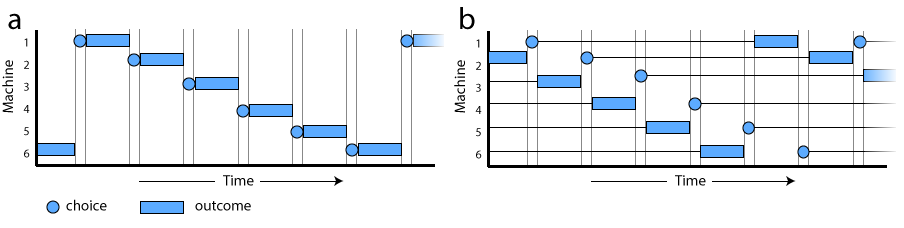
\includegraphics[width=\textwidth]{figures/machinetimeline.png}
\caption{A schematic illustration of the experiment timeline. In all experiments
  and conditions, six 30-second work periods pass between consecutive choices
  with a given machine. \emph{a}: in Experiment 1 and the immediate condition of
  Experiment 2, the outcome for a choice is revealed and occurs immediately
  after the choice is made. \emph{b}: in the delayed condition of Experiment 2 (right),
  the outcome of a choice is revealed and occurs after a delay of four work
  periods.}
\label{fig:machinetimeline}
\end{figure*}



Participants were informed that their job was to perform a monotonous slider task that
would be split into 30-second ``work periods'', but that they would be able to
make choices throughout the experiment that would give them a chance to watch a
Youtube video instead. The number of remaining work periods in the experiment was shown
at the top of the screen, as was the number of seconds left in the current work period.

The slider task was based of a task previously used by \citet{Gill2012}. In each
period of the slider task, five horizontal sliders appeared on the screen (Figure~\ref{fig:taskpictures}\emph{a}). Each
started at a random setting between 0 and 100, with the slider's value
shown to its right, with a random horizontal offset so that the
sliders were not aligned. The participant's task was to use the mouse to move
each slider to ``50'' before the work period ended. When a participant released
the mouse at the correct setting, the slider turned green to show it had been
completed. To ensure that the task took close to the allotted 30 seconds, at the
beginning of the task only the top slider was enabled, and the other four were
grayed out. Additional sliders were enabled at five-second intervals, such that
all five sliders were available after 20 seconds.

Before beginning the experiment, participants chose one of four videos available
on Youtube: an episode of ``Planet Earth'', and episode of ``The Great British
Bakeoff'', and episode of ``Mythbusters'', or an Ellen Degeneres comedy special.
The video was embedded in the experiment with all user controls (such as
skipping ahead) disabled (Figure~\ref{fig:taskpictures}\emph{b}). When given access to the video, participants had to keep the
browser window open and hold down the space bar for the video to play. This allowed us to ensure that
participants maintained engagement with the content.

\begin{figure*}
\centering
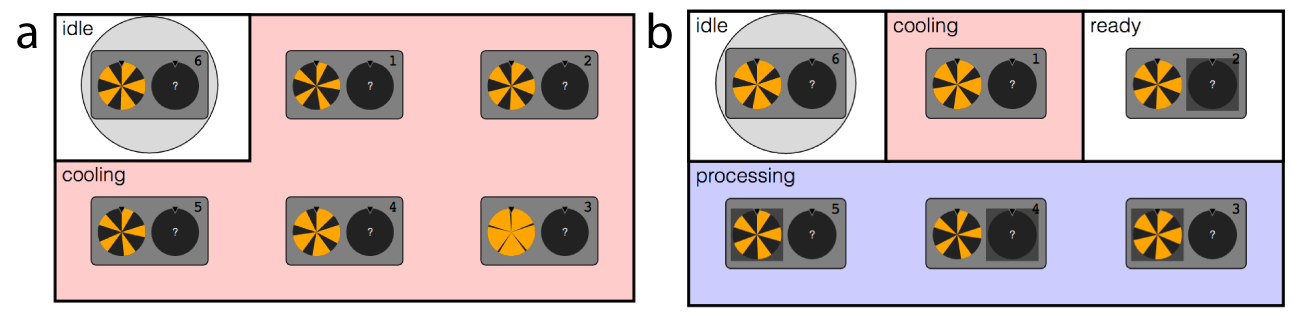
\includegraphics[width=\textwidth]{figures/machinemappictures.png}
\caption{The machine display seen by participants to allow them to keep track of
  the value of each of the six machines and the next time it would be ready to
  make a choice or produce an outcome. \emph{a}: the display seen by
  participants in Experiment 1 and the immediate condition of Experiment 2.
  \emph{b}: the display seen by participants in teh delayed condition of
  Experiment 2.}
\label{fig:machinemappictures}
\end{figure*}

In the main part of the experiment, participants completed a total of 70 work
periods. For the first 10 work periods, participants simply clicked a button to begin the
slider task. After these initial periods, participants gained access to six
``machines'', each of which had a ``current spinner'' and a ``new spinner'' (Figure~\ref{fig:taskpictures}\emph{c}).
Before each work period, participants clicked the circled machine,
were shown the machine and made a choice about which spinner to run. Based on their choices, there was a
chance the machine would perform the work task for the participant, allowing the
participant to watch their chosen video instead.

The machine ran immediately after the choice was
made, and affected the next work period, as shown in
Figure~\ref{fig:machinetimeline}\emph{a} and Figure~\ref{fig:machinemappictures}\emph{a}. It then ``cooled off'' for the
following five periods, as choices were made with the other five machines.

At each choice, participants had to select between two options: run the
machine's ``current spinner'' or run a ``new spinner''. Each machine had two
circular spinners with arrows at the top. The current spinner was split into
five black and five gold wedges. If a participant chose the
current spinner, it spun (immediately or after four periods, depending
on the condition) and, if the arrow landed on the gold wedge, the machine
worked and the participant could watch the video. Initially, the
current spinner's gold wedges were randomly set for each machine to cover between
1/3 and 2/3 of the spinner.

The new spinner initially showed a question mark. If a participant chose the
new spinner, then (immediately or after four periods) a new spinner was
created and appeared on the machine. In the high-explore condition, the new spinner's gold wedges could cover
anywhere from 25\% of the spinner to 100\% of the spinner. In the low-explore condition, the new spinner's gold wedges could cover
anywhere from 0\% of the spinner to 75\% of the spinner. The new spinner then
spun and, if the arrow landed on a gold wedge, the machine worked.
Additionally, if the new spinner had a greater gold area than the current
spinner, the new spinner was ``saved'' and the current spinner was
updated to the new spinner.  This meant that
while choosing a new spinner carried risk, it could carry long-term
benefits as the current spinner could be improved from its initial value.
Importantly, the value of choosing a new spinner was higher in the high-spinner
condition, because the range of outcomes was shifted towards higher values.

Finally, in order to induce exploration throughout the entire experiment, the
six machines would occasionally ``reset'' after they ran. When this occured, a
the current spinner would be set to a new random value between 1/3 and 2/3 gold.
Participants were informed that this would occur randomly on
1/6 of trials. In fact, the procedure was designed so exactly one of the six
machines would reset on each cycle through the machines, and no machine would be
reset on two consecutive uses.

During the machine choices, participants had access to an ``info'' button at the
bottom of the screen that provided reminders about the dynamics of the task. In
addition, before beginning the full experiment, participants completed two
practice phase. First, they performed several trials of practice using the
machines, with the actual work periods removed. Then, they performed three work
periods practicing the slider task.

Participants were given a performance-based bonus of \$3.00 for completing the
slider tasks accurately. If they missed fewer than 10\% of sliders throughout
the experiment and left the video paused less than 20\% of the time, they were
not penalized. However, if they missed more sliders or left the video paused for
longer, they lose 10 cents from their bonus for each additional percentage of
sliders missed or time with the video paused. The running percentage of sliders
missed and video pause time was displayed at the top of the screen throughout
the experiment.

Following the experiment, participants were asked to rate their enjoyment of the
slider task and of the video-watching task on a 1 to 7 scale.


\section{Results}


\begin{figure}
\centering
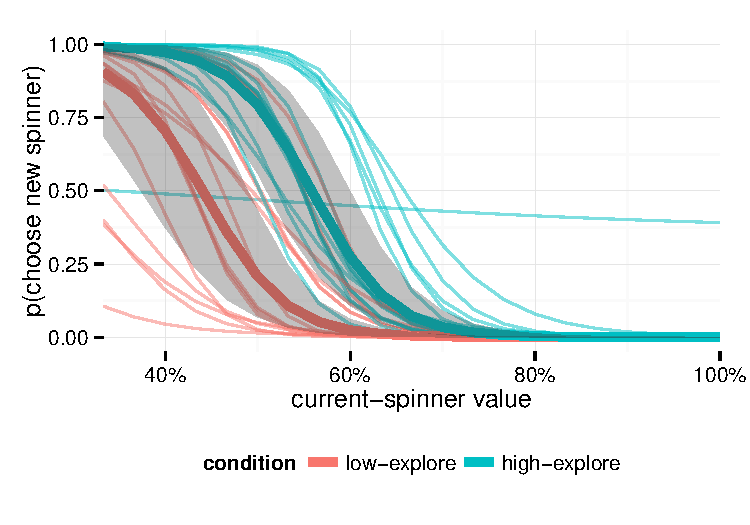
\includegraphics[width=\columnwidth]{figures/exp1results.pdf}
\caption{Model-based estimates of participants' probability of choosing a new
  spinner for different values of the current spinner in Experiment 1. Thick
  lines and shaded regions indicate the mean and 95\% posterior interval for the
  population-level parameters, while the thin lines indicate the mean posterior
  parameters for each of the 31 individual participants. Participants in the
  high-explore condition were more
  likely to explore at a given current-spinner value than those in the
  low-explore condition.}
\label{fig:exp1results}
\end{figure}

Participants rated their enjoyment of the video at 5.77 out of 7, on average,
and their enjoyment of the slider task at 2.87 out of 7, on average. This
difference in enjoyment between the tasks was significant, $t(30)=10.53$, $p<.001$.

To analyze participants trial-by-trial decision-making, we conducted a hierarchical
Bayesian logistic regression using the Stan modeling language \citep{stan-software:2015}.
This approach allowed us to estimate population-level effects of the
current-spinner value and of condition, while also allowing for individual
differences. The regression model included an intercept term as well as terms
for the value of the current spinner, the participant's condition, and a
condition by value of current spinner interaction.

The results of the regression are shown in Figure~\ref{fig:exp1results}.
Because we observed few trails for each participant, and the current-spinner
values observed for each participant depend on chance and the participant's
choices, we present individual-level model fits rather than the raw choice data.
We find that at the population level, participants are less likely to choose a
new spinner when the value of the current spinner is higher, with posterior
probability $p>.999$. We also find that participants in the high-explore are more likely to explore a new spinner for a
given current spinner value than those in the low-explore condition, with
posterior probability $p>.99$. We found no interaction between condition and the
effect of current-spinner value.

\section{Experiment 2}

\subsection{Method}

\subsubsection{Participants.}

Forty participants completed the experiment, which was conducted over
Amazon Mechanical Turk using the psiTurk framework \citep{Gureckis2015a}.
Participants were paid \$5.00 for their participation, with a performance-based
bonus of up to \$3.00. All participants received the full \$3.00 bonus.

\subsubsection{Design and procedure.}

Experiment 2 followed the design of Experiment 1, with the following changes. In
both conditions, the possible winning proportion of a new spinner ranged fro 0\% to 100\% of
the spinner. In the immediate condition the machine ran immediately after the
choice was made, as in Experiment 1. In the delayed condition, each machine was
presented to the participant four work periods before it was schedules to run,
and the participant made a choice at that time. The machine then had to
``process'' for four work periods, thus delaying
the outcome by over 2 minutes. The participant then clicked the machine again to
return to it and observe its outcome, and either perform the slider task or
watch the video. The machine then cooled of for a single period before being
ready for another choice. The timeline for the delayed condition is shown in
Figure~\ref{fig:machinetimeline}\emph{b}.

\section{Results}

\begin{figure}
\centering
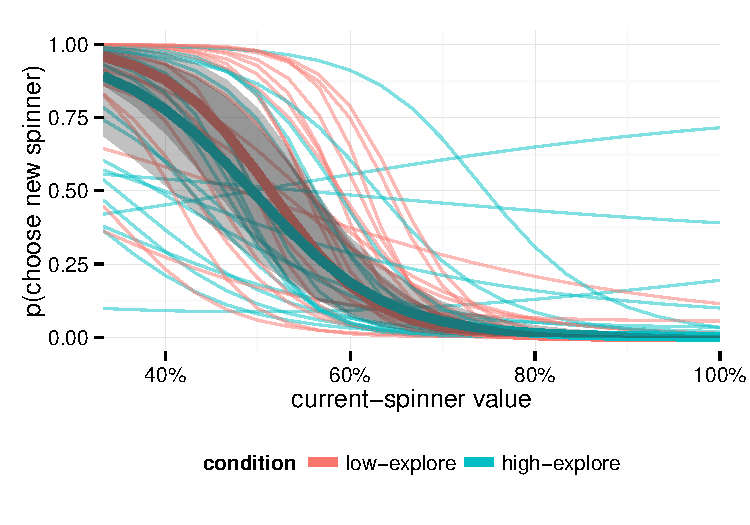
\includegraphics[width=\columnwidth]{figures/exp2results.pdf}
\caption{Model-based estimates of participants' probability of choosing a new
  spinner for different values of the current spinner in Experiment 2. Thick
  lines and shaded regions indicate the mean and 95\% posterior interval for the
  population-level parameters, while the thin lines indicate the mean posterior
  parameters for each of the 40 individual participants. Participants in the
  delayed-outcome condition were no more
  likely to explore at a given current-spinner value than those in the
  immediate-outcome condition.}
\label{fig:exp2results}
\end{figure}

As in Experiment 1, participants rated the video as more enjoyable on average (5.65 out of 7) than the
slider task (3.13 out of 7), $t(39)=9.26$, $p<.001$.

To analyze trial-by-trial decision-making, we conducted a hierarchical Bayesian
logistic regression identical to the one described in the results of Experiment 1.

The results of the regression are shown in Figure~\ref{fig:exp2results}. As in Experiment 1,
participants were less likely to choose a new spinner when the current spinner
has a high value, $p>.999$. However, in this experiment we found no evidence of
an effect of condition, with a posterior probability of $p=.558$ that the effect of condition was
greater than 0. This means that participants were no more likely to explore a new spinner when there
was a temporal delay imposed between their choices and the received outcomes.
However, there may be a small interaction between current spinner value and
condition, such that participants in the delayed condition were less sensitive
to the value of the spinner when making their choices. This might indicate that
the delayed condition was confusing to some participants, as a few individuals
(as seen in Figure~\ref{fig:exp2results}) changed their behavior very little
across current-spinner values. The posterior probability that this interaction
was above 0 is $p=.934$.

\section{Discussion}

In this paper we presented a novel task using immediately-consumed rewards that
may be used to study present bias in the context of exploratory choice. In
Experiment 1 we showed that participants appeared to understand the task and
respond reasonably to maximize their time in the video-watching task. They are
more likely to explore when the current exploitable option (current spinner) has
low value, and change their degree of exploration based on the range of possible
outcomes from choosing a new spinner. However, in Experiment 2 we found that
participants did not explore any more when there was a temporal delay between
choices and outcomes, even though we expected this delay to reduce the present
bias towards the greater immediate rewards of exploitation.

One explanation for our results is that people are in fact less affected by
present bias in the realm of exploratory choice than they are in other
inter-temporal choices.

\begin{small}
  \noindent
\textbf{Acknowledgments} 
\end{small}

\bibliographystyle{apacite}
\bibliography{papers}

\end{document}